\section{Metodología}


\subsection{ACTAR TCP}

El detector ACTAR TPC (\textit{ACtive TARget and Time Projection Chamber}) es un detector diseñado para estudiar núcleos exóticos con tiempos de vida medios muy cortos, que con detectores tradicionales (en los que serían las partículas ligeras las que se acelerarían para bombardear al núcleo de ineterés) sería muy complicado.

Este detector funciona con cinemática inversa, de tal modo que el núcleo pesado es el haz, lo que hace que la cinemática del centro de masas y del laboratorio sea muy diferente, y por tanto su estudio de gran importancia. Además ACTAR TPC es un detector gaseoso, en el que el gas es el medio activo (eseto es, que participa directamente en la reacción de interés). Es gaseoso por varios motivos: el primero es poder usar la ionización de la partícula a través del gas para obtener trazas a partir del rastro de ionización que deja el haz (que sería la parte de la TPC). Bajo la presencia un campo eléctrico los electrones de la ionización derivan hacia el ánodo, recogido por un detector segmentado en pads donde se amplifica su carga. El tiempo de llegada de los electrones $\Delta t$ sirve de estimación de la posición $z$. Otro de los motivos es que las pérdidas de energía son bien conocidas y por tanto corregir errores fácilmente.

Es decir, ACTAR TCP nos permite construcción tridimensionalmente el recorrido de la partícula dentro de la cámara de gas (siendo una de las dimensiones la temporal). Esta recostrucción 3D es la que permite obtener el vértice de la reacción y aplicar correciones por propagación.

Hablando de las características técnicas, la ACTAR TPC tiene una dimensión de $606 \times 606 \times 335 $ mm$^3$, con una caja en el interior de dimensión $295 \times 295 \times 255 $ mm$^3$ llamada cámara de deriva que es precisamente donde está el campo eléctrico  que nos permite recolectar los electrones ionizados (en la parte superior) con detectores de $2 \times 2$ mm$^2$. Nosotros lo llenaremos con una mezcla de dos gases: 90\% D$_2$ e 10\% CF$_4$ a 900 mb (deuterio molecular y tetrafluorometano).

Debido a las pérdidas de energía, existe una cierta probabilidad de que algunas partícuals (principalmente las ligeras) tengan suficiente energía como para atravesar el gas sin pararse, perdiendo información sobre las colisiones. Por eso se disponen a lo largo de los lados de ACTAR y dos muros de silicios justo enfrente a la salida del haz. Los siliiocios tienen un tamaño $5 \times 5$ cm$^2$ $\times 1.5$ mm, y se puede ver la disposición usada en \cref{Fig:Geo_Actar}. Estos silicios tuvieron que colocarse a una distancia prudencial de ACTAR, ya que aunque disminuya la eficiencia de los silicios es posible que el campo eléctrico de los mismos distorsione el campo eléctrico de deriva. Consideraremos la notación l0 y r0 para los silicios de la izquierda y derecha respectivamente y f0  y f1 para la doble capa de silicios en la parte frontal.

\begin{minipage}{0.48\linewidth} \centering
	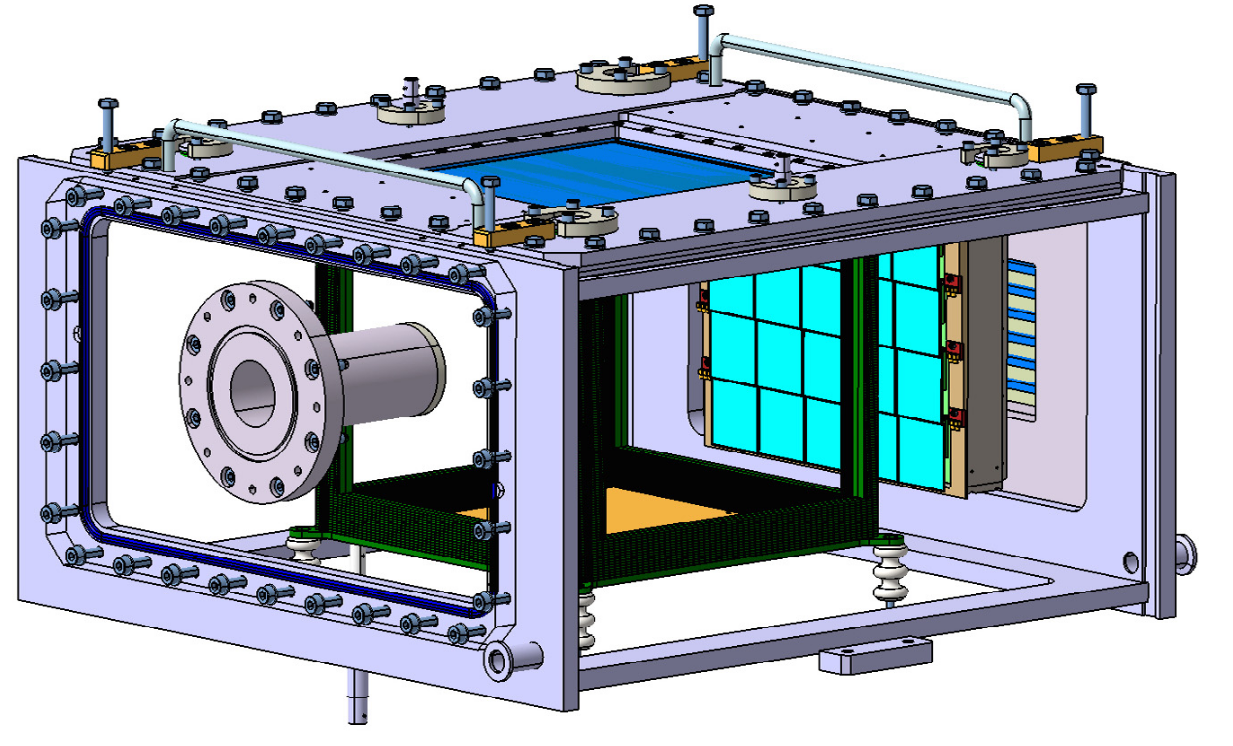
\includegraphics[width=1\linewidth]{Imagenes/ACTAR.png}
	\captionof{figure}{Dibujo en 3D asistido por ordenador (CAD) de (ACTAR TPC). Imagen de \cite{MAUSS2019498}.}
	\label{Fig:ACTAR}
\end{minipage}
\hfill
\begin{minipage}{0.458\linewidth} \centering
	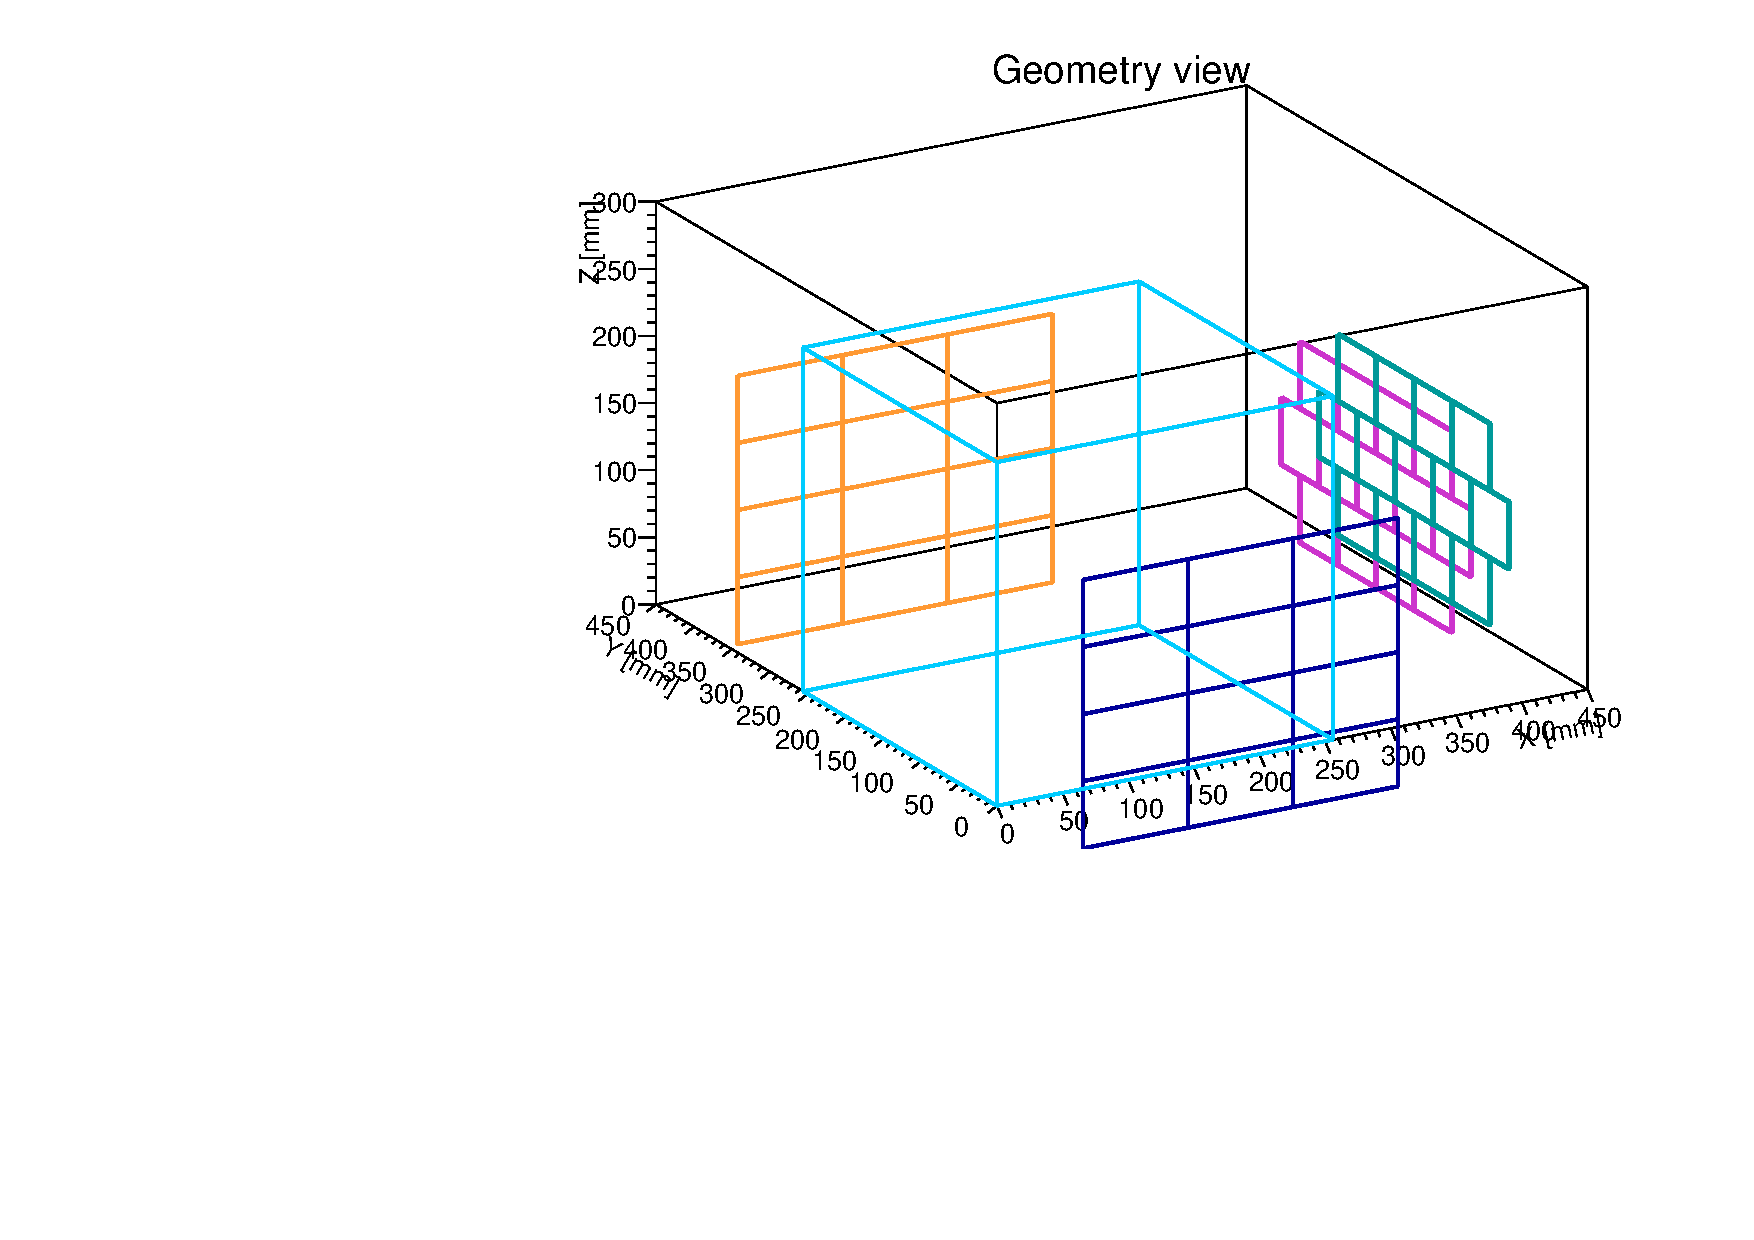
\includegraphics[width=1\linewidth]{Imagenes/Actar.pdf}
	\captionof{figure}{Dibujo de la geometría implementada en la simulacion.}
	\label{Fig:Geo_Actar}
\end{minipage}

\subsection{Cinemática} \label{Subsec:03-cinematica}

En este apartado trataremos de resolver la cinemática de la reacción de interés $^{11}\text{Li}(d,t)^{10}\text{Li}$. Resolver la cinemática basicamente implica obtener los ángulos de las partículas salientes y sus energías en función de: la energía cinética de la partícula incidente en el sistema laboratorio, el ángulo del centro de masas (que es el afectado por la sección eficaz) y la energía de exctiación de la partícula $^{10}$Li (o la energía de excitación en general que podrá llevar también la ligera).

La cinemática responde únicamente a las leyes de conservación de la energía-momento, por lo que no tendremos que tener en cuenta ni interacciones electromagnéticas ni nucleares. La sección eficaz que influye en el ángulo de salida, que encierra la física nuclear de la interacción, será discutida más adelante.

\subsubsection{Notación}
Dado que en función del sistema de referencia tendremos un valor de momento u otro, necesitaremos especificar que sistema de referencia seguimos. Usaremos las siguiente notación: $p_{1}$ es el momento en el sistema laboratorio y $p_{1}'$ es el sistema del centro de masas. En la siguiente figura presentamos un esquema de ambos sistemas de referencia, y como son las partículas para cada uno de ellos.

\begin{minipage}[t]{0.45\linewidth}
	\begin{center}
		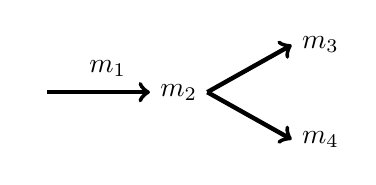
\begin{tikzpicture}[thick,scale=0.6]
			\node (1) at (-3,0) {};
			\node (2) at (0,0) {$m_2$};
			\node (3) at (3,1) {$m_3$};
			\node (4) at (3,-1) {$m_4$};
			\node (m1) at (-1.5,0.5) {$m_1$};
			\draw[arrows={->},ultra thick] (1.east)--(2.west);
			\draw[arrows={->},ultra thick] (2.east)--(3.west);
			\draw[arrows={->},ultra thick] (2.east)--(4.west);
		\end{tikzpicture}
		\captionof{figure}{Sistema Laboratorio}
	\end{center}
\end{minipage}
\hfill
\begin{minipage}[t]{0.45\linewidth}
	\begin{center}
		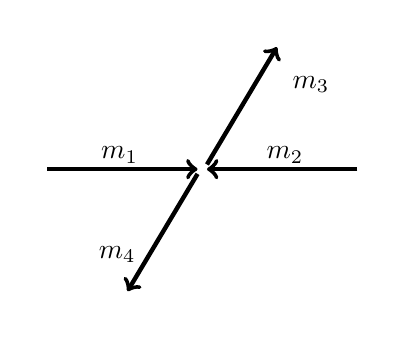
\begin{tikzpicture}[thick,scale=0.6]
			\node (1) at (-3.5,0) {};
			\node (2) at (3.5,0) {};
			\node (3) at (1.8,2.8) {};
			\node (4) at (-1.8,-2.8) {};
			\draw[arrows={->},ultra thick] (1.east)--(-0.1,0)  ;
			\draw[arrows={->},ultra thick] (2.west)--(0.1,0)  ;
			\draw[arrows={->},ultra thick] (0.1,0.1)--(3.south west)  ;
			\draw[arrows={->},ultra thick] (-0.1,-0.1)--(4.north east)  ;

			\node (m1) at (-1.75,0.3) {$m_1$};
			\node (m2) at (1.75,0.3) {$m_2$};
			\node (m3) at (2.3,1.8) {$m_3$};
			\node (m4) at (-1.8,-1.8) {$m_4$};
		\end{tikzpicture}
		\captionof{figure}{Sistema Centro de Masas}
	\end{center}
\end{minipage}

\subsubsection{Cálculo de los ángulos}
En esta sección trataremos de obtener los ángulos de salida de las partículas 3 y 4 (y sus energías) en función de las variables conocidas: energía cinética y masas de las partículas. Para esto necesitaremos calcular las energías de las partículas en el sistema centro de masas, ya que las relaciones de conservación de la energía es mucho mas sencilla en este sistema referencial. Luego podremos recuperarlas usando la \textit{transformada de Lorentz}.

Como podemos ver en las figuras, en el sistema laboratorio la partícula 1 está en movimiento mientras que la partícula 2 está en reposo. Eso nos lleva a que sus momentos, en el sistema de referencia del laboratorio:

\begin{eqnarray}
	P_1 = (E_1/c,\pn_1) & \quad P_2 = (m_2c,0) \\
	P_3 = (E_3/c,\pn_3) & \quad P_4 = (E_4/c,\pn_4)
\end{eqnarray}
Por otro lado, los momentos en el sistema de referencia del centro de masas vendrán dados por

\begin{eqnarray}
	P_1' = (E_1'/c,\pn_1') \quad P_2 = (E_2'/c,-\pn_1') \\
	P_3' = (E_3'/c,\pn_3') \quad P_4 = (E_4'/c,-\pn_3')
\end{eqnarray}
Asumiremos que la partícula 1 incidente se mueve únicamente en el eje $x$ tal que $\pn_1=(p_1,0,0)$. En ese caso el sistema centro de masas se moverá respecto al sistema laboratorio en el eje $x$, por lo que habrá que aplicar la transformaciones de Lorentz (\ref{Ec:04} y \ref{Ec:05}) siendo válidas para \textit{cualquier cuadrimomento}. Definimos las energías totales como $E_{tot}=E_1+E_2$ y como  $E_{tot}'=E_1'+E_2'$, siendo esta última la \textit{energía del centro de masas}, que verifica que
\begin{equation}
	E_{tot}' \equiv E_{CM} = E_{tot}^2 - c^2p_1^2 \label{Ec:18}
\end{equation}
Tanto $E_{tot}$ como $E_{tot}'$ son variables conocidas. Nos interesa calcular las energías $E_3'$ y $E_4'$, que usando la transformación de Lorentz nos servirán para estudiar las energías $E_3$ y $E_4$, así como los momentos. Las relaciones se pueden calcular como

\begin{equation}
	E_c' = E_{tot}' - E_{ex}
\end{equation}
siendo $E_{ex}$ la parte de la energía inicial que se convierte en energía de estados excitados de las partículas 3 y 4. Así pues:
\begin{eqnarray}
	E_3 ' & = & \frac{1}{2} \left( E_{c}' + \frac{m_3^2c^4- m_4^2c_4}{E_{c}'} \right) \\
	E_4 ' & = & \frac{1}{2} \left( E_{c}' + \frac{m_4^2c^4- m_3^2c_4}{E_{c}'} \right)
\end{eqnarray}
A partir de estos valores de $E_3'$ y $E_4'$ podemos calcular el valor de los momentos $p_3'$ y $p_4'$ (en módulo). Podemos suponer sin ningún tipo de problema que la coordenada $x$ de los momentos vienen dadas por

\begin{eqnarray}
	p_{3x}' = p_3' \cos (\theta_3') \\
	p_{4x}' = p_4' \cos (\theta_4')
\end{eqnarray}
de este modo podemos aplicar las transformaciones de Lorentz para hallar los valores del $\cos (\theta_3)$ y $\cos (\theta_4)$. Así:

\begin{eqnarray}
	p_3 \cos (\theta_3) = \gamma (p_3' \cos (\theta_3')+\beta E_3'/c)
\end{eqnarray}
despejando $\cos (\theta)$ obtenemos:

\begin{equation}
	\cos (\theta_3) = \frac{\gamma}{p_3} (p_3' \cos (\theta_3')+\beta E_3'/c)
\end{equation}
El cálculo de $p_4$ es exactamente igual, obteniendo


\begin{equation}
	\cos (\theta_4) = \frac{\gamma}{p_4} (p_4' \cos (\theta_4')+\beta E_4'c)
\end{equation}
En la siguiente gráfica \ref{Fig:04-Kin} podemos ver la dependencia entre el ángulo $\theta_3$ y $\theta_4$ y la energía cinética de salida, en la que podemos ver una función que las relaciona unequívocamente.

\begin{figure}[H] \centering
	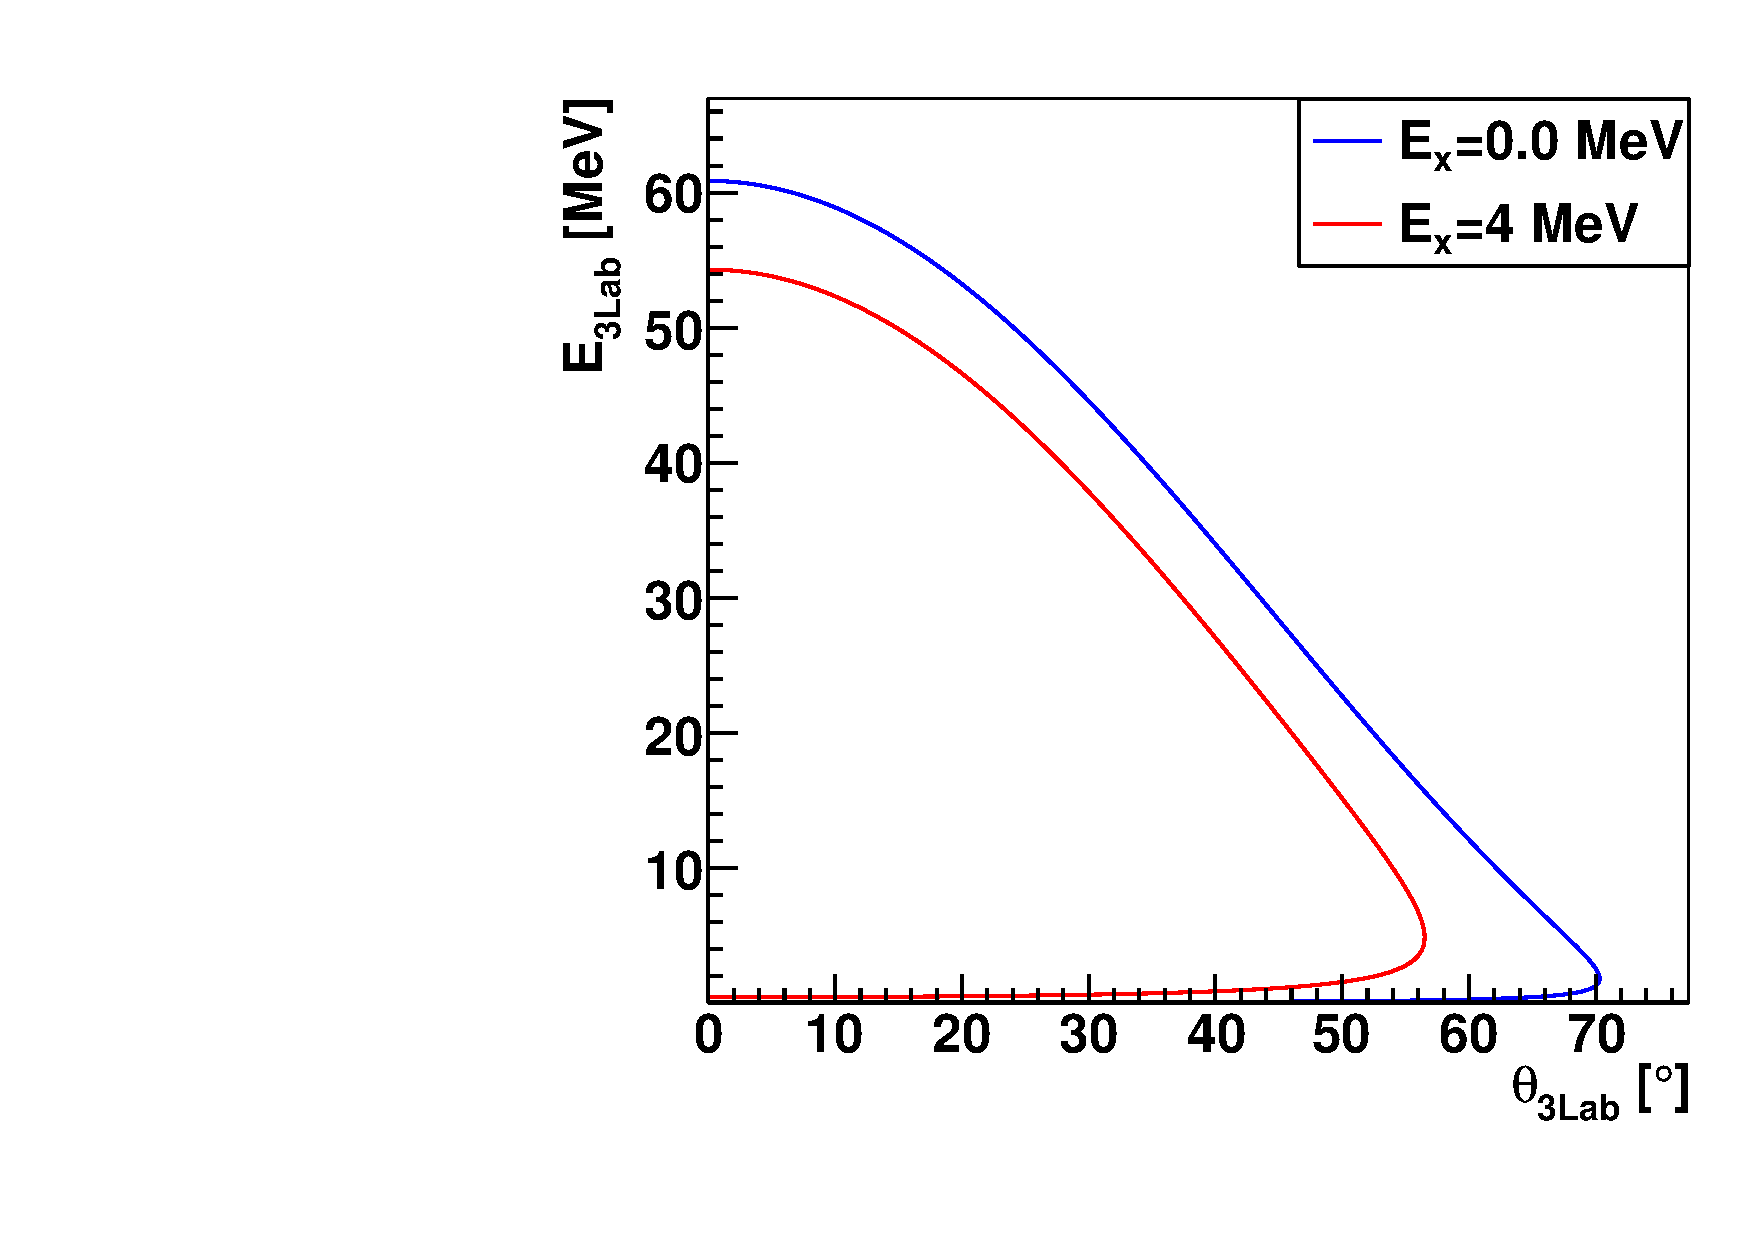
\includegraphics[width=0.7\linewidth]{Imagenes/Cinematica.pdf}
	\caption{Cinemática de la reacción $^{11}\text{Li}(d,t)^{10}\text{Li}$, donde se muestra la energía cinética del tritio (izquierda) y del $^{10}$Li (derecha) frente su ángulo de salida.}

	\label{Fig:04-Kin}
\end{figure}


\subsection{Pérdidas de energía en el Gas}

Las pérdidas de energía en el gas son sumamente importantes en el estudio de un dector gaseoso, ya que tendrán que ser tenidas en cuenta a la hora de recuperar la energía en el centro de masas de las partículas ligeras, fundamental para saber si el litio está en un estado excitado. La mejor manera de caracterizar la pérdida de energía de una partícula por un medio gaseoso viene dada por la \textbf{ecuación de Bethe} (en nuestro caso usarmeos la aproximación no relativista), que nos dice que el poder de frenado lineal $S$, definido como la pérdida de energía de la partícula dividida por la longitud diferencial de la trayectoria  \cite{Knoll:1300754}


\begin{equation}
	S = - \frac{dE}{dx} \simeq \frac{4 \pi e^4}{m_e} \left( \rho \frac{N_A}{M} \right) \frac{z^2 Z}{v^2} \ln \left( \frac{2 m_e v^2}{I} \right)
\end{equation}
donde $z$ es el número atómico incidente, $Z$ la de la partícula absorbente, $v$ la velocidad de la partícula incidente, $N_A$ el número de avogadro, $M$ la masa atómica del gas, $\rho$ su densidad (por lo que dependerá de la presión, un input interesante) e $I$  representa el potencial promedio de excitación e ionización del absorbedor. Se trata como un parámetro determinado experimentalmente para cada elemento.

Dado que nuestra cámara de gas estará formada por una mezcla de gases, la ecuación de la pérdida no será exactamente la anterior, si no que responderá a la \textit{regla de Bragg-Kleeman} \cite{Knoll:1300754}

\begin{equation}
	\frac{1}{N_c} \left( \frac{dE}{dx} \right)_c = \sum_i W_i \, \frac{1}{N_i} \left( \frac{dE}{dx} \right)_i
\end{equation}
siendo $W_i$ el peso del gas $i$ y $N_i$ la densidad atómica tal que $N_i = \rho N_A
	/ M_i$.

El valor de \( -dE/dx \) a lo largo de la trayectoria de una partícula también se llama su \textit{pérdida específica de energía}, una ``tasa'' de pérdida de energía. En realidad esta ecuación es puramente estadística, ya que cada colisión entre el átomo y los electrónes del gas es pequeña, y por tanto nosotros usamos promedios. Al ser un fenómeno estadístico, existe un error indefectible tanto en la simulación como en la recuperación de la energía cinética. A estas fluctuaciones debido a su naturaleza estocástica en la energía cinética las llamadmos \textbf{straggling}, lo que hace que no todas las partículas con una misma energía se paren a la misma distancia. Este straggling tendrá que ser tenido muy en cuenta ya que son un factor de incertidumbre de la energía cinética muy grande. Otras definición de interés es el \textbf{rango}, que para una energía perdida conocida nos permite calcular la distancia media recorrida y el \textbf{punch-trough}, que nos da para una energía inicial de la partícula la distancia máxima que puede recorrer en ese medio.


\subsection{Detectores}

Los detectores de silicio están formadas por uniones PN en los que la partícula incidente genera pares de electrones-hueco que gracias a la presencia de una pequeña coriente eléctrica y un alto campoeléctrico son inmediantamente separadas evitando la recombinación, de tal modo que la intensidad de la corriente. La intesidad de la corriente generada estará relacionada con la energía depositada.

Al igual que con la interacción partícula-gas, las pérdidas de energía a través de la generación de pares de portadores respoe a fenómenos estocásticos, y como tal introduce un error estadístico intrínseco a la medida de energía de los silicios, que nosotros en la simulación debemos considerar. La manera de tener en cuenta este fenómeno se hace a través de la resolución intrínseca del semiconductor.


La \textbf{resolución energética intrínseca} $R$ estará relacionada con el FWHM de la distribución estadística de la energía depositada en el silicio por parte de la partícula para la energía de dicha particula, de tal modo que:

\begin{equation}
	\text{FWHM} = R \cdot E
\end{equation}
y dado que $\sigma = 2.35 \text{FWHM} $, tenemos que la $\sigma$ de la distribución gaussiana que parece seguir la energía depositada es:

\begin{equation}
	\sigma  = \frac{R \cdot E}{2.35}
\end{equation}
Ahora bien, la resolución intrínseca, en el caso de los detectores semiconductor dependenj del número de portadores de carga y del \textit{factor de Fano}. A pesar de numerosos experimentos, el factor de Fano tanto para el silicio como para el germanio aún no está bien determinado. Sin embargo, está claro que \( F \) es pequeño, en el orden de 0{.}12. La \textbf{resolución esperada} es \cite{Leo:302344}

\begin{equation}
	R = 2.35 \sqrt{\frac{F}{J}} = 2.35 \sqrt{\frac{F w}{E}}
\end{equation}
donde \( w \) es la energía promedio para la creación de un par electrón-hueco, y \( J = E/w \). El valor de la creación de un par electrón-hueco depende del tipo de semiconductor y de lat temperatura. Por ejemplo para el silicio tenemos $w=3.62$ eV para una $T=$300 K mientras que $w=3.81$ eV si $T=77$ K. Nosotros usamos valores experimentales usadas con nuestras partículas. En particular nosotros sabemos que para una energía de 5.5 MeV de nuestras parículas al atravesar el semiconductor contamos con una resolucion de $50$ keV, tal que la $\sigma$ que vamos a usar en la simulación para parametrizar la energía deposiada en los silicios viene dada por:

\begin{equation}
	\sigma = \frac{0.0213}{2.35} \sqrt{E} \ \unit{MeV} \label{Ec:03-resolucion}
\end{equation}
Las especificaciones técnicas de los silicios están detalladas en   \cite{MAUSS2019498}. , donde se nos dice que los detectores de silicio se encuentran acoplados a un preamplificador de carga sensible con una sensibilidad de 10 mV/MeV, seguido de un amplificador CAEN N568 configurado con un tiempo de moldeado de 3 $\mu$s y una ganancia de $\times 32$.

\subsection{Sttragling Angular}

Gracias a la TPC podemos reconstruir la traza del tritio que nos da información acerca del ángulo $\theta_{lab}$ de las partículas resultantes de una interacción. También podemos obtenerla  a partir del vértice de interacción, la dirección del haz y el punto de interacción con el impacto del silicio. Debido a las dimensiones del pad en los que se recoge la carga y la propia resolución del silicio, en ambos casos se tiene una resolución similar. La distribución de cada medida de $\theta_{lab}$ sería una gaussiana con FWHM = 1$^{\circ}$, que será, tal y como veremos, el factor que generá mas anchura $\sigma$ en las distribuciones de energía.